\subsection{Perceived Randomness}\label{subsection:perceived_randomness}
\subsubsection{Are Humans Good Randomisers?}\label{subsubsection:are_humans_good_randomisers}
The definition of the term ``random'' is a contentious area for debate. In essence, randomness is an unobservable characteristic of a generating process therefore the act of trying to define it is somewhat contradictory. To determine if a process or sequence is random, it has to be put through statistical tests for specific properties which are deemed to be ``random''. However, because these tests are statistical, are the conclusions drawn \textit{objectively} random or purely \textit{subjective}?

Research into the human perception and generation of random sequences is a common topic within psychological papers yet the contradictory nature of findings results in a less-than-satisfactory answer to the question of ``Are humans good randomisers?'' \textendash{} much like when defining the term itself.

The origins of such a question can be traced back to an observation made by Hans Reichenbach in The Theory of Probability~\cite{reichenbach:1949}; he suggested that when asked to produce a series that seemed random to them, people untrained in the theory of probability would be unable to generate such a series and, instead, generate one that would contain patterns and biases, e.g.\ too many alternations than what was expected. This ultimately suggests that humans are not good randomisers which is the prevalent opinion to date. This behaviour is attributed to the fact that human-generated sequences often reflect the underlying psychological tendencies of subjects, rather than the unpredictability of true randomness.

While Reichenbach takes the stance that humans are not good randomisers, the alternative to this conclusion was put forward by the work of Bruce Ross~\cite{ross:1955}. Ross explores the processes involved in randomising binary sequences and analyses the methods that people use, as well as the typical mistakes that they make when attempting to create random sequences. In his study, Ross got 60 subjects to stamp cards with either an `$\mathcal{O}$' or an `$\mathcal{X}$' and place them singly in a $100$-item sequence that they thought to be random in the middle of a table, with item frequencies of either $50-50$, $60-40$, or $70-30$. These sequences were then scored against the expected properties of a random sequence and, based on the analysis conducted, resulted in ``the prevalent \textit{a priori} assumption that the human being is a systematically biased randomi[s]er [not being] borne out''~\cite{ross:1955} and that ``[subjects] who are instructed to construct a random series give a fairly good approximation of the expected number of alternations''~\cite{bakan:1960}. This, however, is not sufficient to deem that humans are not systematically biased randomisers.

\subsubsection{Judgement vs. Production of Random Binary Sequences}\label{subsubsection:judgement_vs_subsection:production_of_random_binary_sequences}
As alluded to by the question posed in the previous subsection, the human perception of randomness is a \textit{subjective}, rather than \textit{objective}, quality. Because of this subjectivity, it will vary from person to person and two natural conclusions can be drawn from this—either that people have an incorrect idea of what randomness is and what it should look like, or that people intuitively know what true randomness should look like, but there is some internal functional limitation that prevents the judgement and production of such sequences~\cite{wagenaar:1970}, being so powerful that individuals may choose to forego an available statistical analysis in favour of this `gut feeling'~\cite{bar-hillel:1991}.

Being that the topic of this dissertation is Prediction with Expert Advice, specifically in the scenario of $\eta$-mixable Games—a subject to be introduced in the following section—the primary focus of this literature review will be centred around experiments conducted to explore the judgement and production of random binary sequences. These two categories both make interesting observations about the internal mechanism responsible for the human perception of randomness, namely ``that [humans] see clumps or streaks in truly random series and expect more alternation, or shorter runs, than are there'', and that ``[humans] produce series with higher than expected alternation rates''~\cite{bar-hillel:1991}.

\paragraph{Judgement of Random Binary Sequences}\label{paragraph:judgement_of_random_binary_sequences}
We will first explore \textit{judgement}. In Willem Wagenaar's study titled ``Appreciation of conditional probabilities in binary sequences'', Wagenaar examines how people perceive and interpret the likelihood of certain events occurring given previous outcomes revealing a disparity between what was perceived to be random and what was truly random, as well a systematic recency bias that affected subject's judgements of conditional probabilities~\cite{wagenaar:1970}. The study controlled the conditional probability of a $0$ after $0$ ($1$ after $1$) as the experimental variable, testing it between the range $0.2-0.8$ with $0.1$ increments, i.e. 7 values, for first-, second-, and third-orders of dependency. To test this, subjects were shown 16 sets of 7 binary sequences (each generated with one of the conditional probabilities in the range) for each order of dependency and were asked to select and record the sequence in each set that looked the most random to them—explained as the sequence that looked the most likely to be produced when flipping a fair coin.

For reference, in a truly random binary sequence, the conditional probability of $0$ after $0$ ($\text{Pr}(0|0)$) or $1$ after $1$ ($\text{Pr}(1|1)$) for the first order of dependency is $0.5$. However, Wagenaar identified sequences with conditional probabilities close to $0.4$ were the ones perceived as the most random across all orders of dependency, affirming the position that humans aren't good randomisers. This study also highlights the bias in favour of `negative recency', more commonly known as the gambler's fallacy wherein gamblers will tend to bet on red after a run of blacks (and vice versa) on a roulette wheel. This observation ultimately caused subjects to favour series with slightly more alternations than is expected of true randomness causing Wagenaar to postulate that this is because subjects ``cannot process such a mathematical quantity as `conditional probability'\ldots Rather, they will look at some other characteristics like, for instance, the run-structure of the sequence''~\cite{wagenaar:1970}.

\paragraph{Production of Random Binary Sequences}\label{paragraph:production_of_random_binary_sequences}
Having introduced the topic and a systematic bias that affects how humans judge sequences to be random, we can now delve into generation\textemdash{}the category that this project will explore.

Examining Paul Bakan's work titled ``Response-Tendencies in Attempts to Generate Random Binary Series'', Bakan aimed to ``allow for another test of the hypothesis that [a subject] will generate more runs than chance predicts under conditions somewhat different from those reported by Ross'' in that biases in motor operations (e.g., favouring to use their dominant hand) was avoided~\cite{bakan:1960}. As stated by Bakan, the main findings of this study are that subjects ``exhibit consistent patterns of responses'' and ``deviate from randomness by having too many alternations in the series'' when trying to generate a random binary sequence—a conclusion supported by~\cite{lopes:1987}: ``humans-produced sequences have too few symmetries and long runs, too many alternations among events, and too much balancing of event frequencies over relatively short regions'' which may be explained by the fact that a human's short-term memory roughly spans 7 (+/- 2) items that constitute the ``window'' that people try to achieve representative randomness in~\cite{kubovy:1988}.

Lastly, we explore the work of Raymond Nickerson and Susan Butler titled ``On producing random binary sequences'' which forms the basis of the experiment that this project will carry out. Nickerson and Butler's experiment varies from previous ones carried out in that, instead of getting subjects to produce a single sequence that would later be aggregated into a larger collective, they got subjects to produce several sequences while attempting to be random since they noted that ``randomness does not reveal itself in any single short sequence; it reveals itself in sets of such sequences. Or at least it has a better opportunity to reveal itself in a set of sequences rather than in a single member of such a set.''~\cite{nickerson:2009}. In their methodology, subjects were tasked with producing 100 10-item random sequences—explained as the sequences likely to be recorded if 100 individuals were asked to flip a fair coin 10 times each—that would be statistically indistinguishable from if an actual coin were to have been flipped. The notion behind this experiment was that, if subjects' perceptions of randomness were good, then subjects would be able to produce sets of sequences with properties (i.e., number of heads per sequence, number of runs per sequence, run lengths, frequency of alternations and repetitions) that fell within expected percentages. Because each subject was made to produce several sequences, their results provided a stronger justification for a human's ability as a randomiser since it allows subjects time to prove that they can act randomly. What Nickerson and Butler found was that, while subjects weren't any good at producing truly random sequences since ``in the aggregate, the sets of sequences produced by our participants differed quantitatively from those expected of a random process, so our results can be seen as supporting the prevailing view that people are not very good randomi[s]ers'', the distribution shape produced by the aggregate of participants' sequences were qualitatively similar—``not indistinguishable, but close''~\cite{nickerson:2009}\textemdash{}to what was expected (shown in the figures below), suggesting that humans can be effective randomisers when part of a group.
\begin{figure}[h]
    \centering
    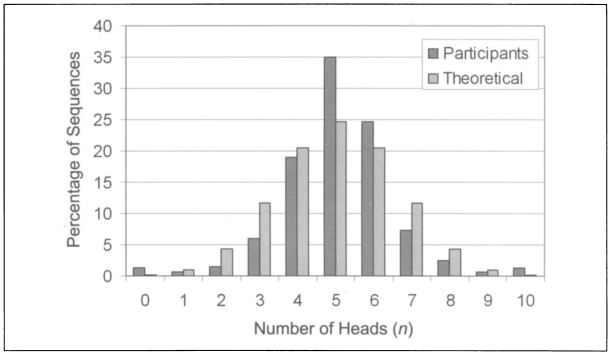
\includegraphics[width=0.9\textwidth]{images/nickerson_2009_number_of_heads.png}
    \caption{Percentage of 10-toss sequences with $n$ heads, including the theoretical distribution, $X \sim B(10, 0.5)$, for comparison~\cite{nickerson:2009}.}
\end{figure}

\begin{figure}[ht]
    \centering
    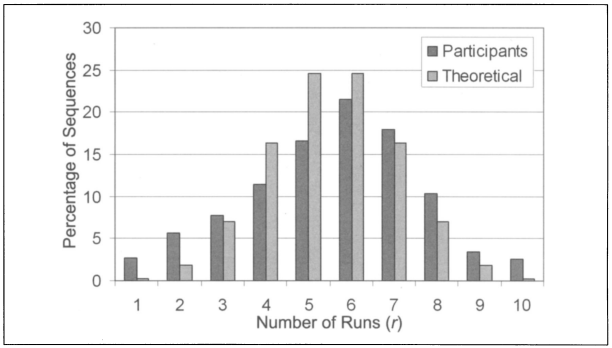
\includegraphics[width=0.9\textwidth]{images/nickerson_2009_number_of_runs.png}
    \caption{Percentage of all 10-toss sequences with $r$ runs, including the theoretical distribution for comparison~\cite{nickerson:2009}.}
\end{figure}